\documentclass[utf8]{frontiersSCNS}

\setcitestyle{square}
\usepackage{url,hyperref,lineno,microtype,subcaption}
\usepackage[onehalfspacing]{setspace}

\usepackage{bm}
\usepackage[ruled,vlined]{algorithm2e}
\usepackage{graphicx}
\usepackage{amsmath}
\usepackage{amssymb}
\usepackage{mathtools}
\usepackage{adjustbox}
\usepackage{array}

\newcommand{\mtx}[1]{\bm{#1}}
\DeclareMathOperator*{\minimize}{minimize}
\newcolumntype{L}{>{\centering\arraybackslash}m{.3\textwidth}}
\renewcommand{\arraystretch}{1.4}

\linenumbers

\def\keyFont{\fontsize{8}{11}\helveticabold }
\def\firstAuthorLast{Gammell {et~al.}}
\def\Authors{Jimmy Gammell\,$^{1,*}$, Sonia Buckley\,$^{1}$,Sae Woo Nam\,$^{1}$ and Adam N. McCaughan\,$^{1}$}
\def\Address{$^{1}$National Institute of Standards and Technology, Boulder, CO, United States}
\def\corrAuthor{Jimmy Gammell}
\def\corrEmail{jimmy.gammell@colorado.edu}

\begin{document}
\onecolumn
\firstpage{1}

\title[Layer-skipping connections]{Layer-skipping connections facilitate training of layered networks using equilibrium propagation.} 

\author[\firstAuthorLast ]{\Authors}
\address{}
\correspondance{}

\extraAuth{}% If there are more than 1 corresponding author, comment this line and uncomment the next one.
%\extraAuth{corresponding Author2 \\ Laboratory X2, Institute X2, Department X2, Organization X2, Street X2, City X2 , State XX2 (only USA, Canada and Australia), Zip Code2, X2 Country X2, email2@uni2.edu}


\maketitle


\begin{abstract}
\section{}
Equilibrium propagation is a learning framework that marks a step forward in the search for a biologically-plausible implementation of deep learning, and could be implemented efficiently in neuromorphic hardware. Previous applications of this framework to layered networks encountered a vanishing gradient problem that has not yet been solved in a simple, biologically-plausible way. In this paper, we demonstrate that the vanishing gradient problem can be overcome by replacing some of a layered network's connections with random layer-skipping connections. We additionally compare the computational complexities of equilibrium propagation and backpropagation to show that it would be easier to implement the former in neuromorphic hardware.

\tiny
 \keyFont{ \section{Keywords:} equilibrium propagation, deep learning, small-world, layer-skipping connections, neuromorphic computing, biologically-motivated}
 
\noindent\textbf{Number of words:} 6417

\noindent\textbf{Number of figures:} 7

\noindent\textbf{Number of tables:} 1
\end{abstract}

\section{Introduction}

As research into neural networks grows, there has been increased interest in designing biologically-inspired training algorithms, as they may offer insight into biological learning processes and also offer clues towards developing energy-efficient neuromorphic systems \citep{wozniak2018, crafton2019, ernoult2020, bartunov2018, lillicrap2014, bengio2015}. The equilibrium propagation learning framework developed \cite{scellier17} is one such algorithm.  It is a method for training a class of energy-based networks, the prototype for which is the continuous Hopfield network \cite{hopfield1984}.  In particular, it addresses one of the major issues that prevent other training algorithms (such as backpropagation) from being biologically-plausible, which is the requirement for separate computation pathways for different phases of training. This also makes the algorithm appealing for practical implementation into neuromorphic hardware, because only a single computation circuit is required within each (non-output) neuron, rather than multiple distinct circuits. However, current implementations of the algorithm still have a defect that diminishes its biological plausibility: they require hand-tuned per-layer hyperparameters to account for a vanishing gradient through the network. In addition to not being biologically plausible, these multiplicative hyperparameters would be difficult to implement in a neuromorphic hardware system with limited bit depth. In this work, we demonstrate that the vanishing gradient problem can instead be solved through topological means: by randomly replacing some of a layered network's connections with layer-skipping connections, we can generate a network that trains each layer more evenly and does not need per-layer hyperparameters.


Implementation of equilibrium propagation in \citep{scellier17} was hindered by a vanishing gradient problem whereby networks with as few as 3 hidden layers trained slowly on MNIST \citep{mnist1998} -- a serious issue given that network depth is critical to performance on difficult datasets \citep{simonyan2014, srivastava2015tvdn} and that convergence to a low error rate on MNIST is a low bar to meet. The problem was overcome in \citep{scellier17} by independently tuning a unique learning rate for each layer in the network.  These learning rates were multiplicative factors that proportionally scaled the signals communicated between layers.



In our work, we have modified the strictly-layered topology of the original implementation by adding and removing connections to create a small-world network\citep{watts98}. Through this modification we have eliminated the per-layer hyperparameters without degrading the algorithm's performance -- the modified network produces 0\% training error (out of 50,000 examples) and $\lesssim$2.5\% test error (out of 10,000 examples) on MNIST using a network with three hidden layers and no regularization term in its cost function. These error rates are comparable to those of other biologically-motivated networks \citep{bartunov2018} and are approximately the same as those of the layered network with unique, manually-tuned learning rates in \citep{scellier17}. Our method could be implemented with relative ease in any system with configurable connectivity, such as those already described in several neuromorphic hardware platforms \citep{davies2018, schemmel2010, shainline2019}. Layer-skipping connections have been observed in biological brains \citep{bullmore2009}, so the approach is biologically-plausible. Similar techniques have seen success in convolutional \citep{he2015, srivastava2015} and multilayer feedforward \citep{xiaohu2011, krishnan2019} networks. Our findings outlined in this paper suggest that layer-skipping connections are effective-enough to be appealing in contexts where simplicity and biological plausibility are important.

\section{Background}

\subsection{Equilibrium propagation}
\label{sec:eqp_formulation}

Similarly to backpropagation, the equilibrium propagation algorithm \citep{scellier17} trains networks by approximating gradient descent on a cost function. Equilibrium propagation is applicable to any network with dynamics characterized by evolution to a fixed point of an associated energy function; our implementation is a recreation of that in \citep{scellier17}, which applies it to a continuous Hopfield network \citep{hopfield1984}. The mathematical formulation of the framework can be found in \citep{scellier17}. We discuss its appeal over backpropagation in section \ref{sec:comparison}.

\subsubsection{Implementation in a continuous Hopfield network}

Here we summarize the equations through which a continuous Hopfield network is trained using equilibrium propagation; this summary is based on the more-thorough and more-general treatment in \citep{scellier17}.

Consider a network with $n$ neurons organized into an input layer with $p$ neurons, hidden layers with $q$ neurons and an output layer with $r$ neurons. Let the activations of these neurons be denoted respectively by vectors $\mtx{x}\in\mathbb{R}^{p}$, $\mtx{h}\in\mathbb{R}^{q}$ and $\mtx{y}\in\mathbb{R}^{r}$, and let $\mtx{s}=(\mtx{h}^{T},\mtx{y}^{T})^{T}\in\mathbb{R}^{q+r}$ and $\mtx{u}=(\mtx{x}^{T}, \mtx{s}^{T})^{T}\in\mathbb{R}^{n}$ be vectors of, respectively, the activations of non-fixed (non-input) neurons and of all neurons in the network. Let $\mtx{W}\in\mathbb{R}^{n\times n}$ and $\mtx{b}\in\mathbb{R}^{n}$ denote the network's weights and biases where $w_{ij}$ is the connection weight between neurons $i$ and $j$ and $b_i$ is the bias for neuron $i$ ($\forall i \;w_{ii}=0$ to prevent self-connections), and let $\rho$ denote its activation function; here and in \citep{scellier17},
\begin{equation}
\rho(x)=\begin{cases}0&x<0\\x&0\leq x\leq 1\\1&x>1\end{cases} \label{eqn:hardened_sigmoid}
\end{equation}
 is a hardened sigmoid function
where $\rho'(0)=\rho'(1)$ is defined to be 1 to avoid neuron saturation. Let $\mtx{\rho}((x_1,\hdots, x_n)^T)=(\rho(x_1),\hdots,\rho(x_n))^T$.

The behavior of the network is to perform gradient descent on a total energy function $F$ that is modified by a training example $(\mtx{x}_d,\mtx{y}_d)$. Consider energy function $E:\mathbb{R}^n\to\mathbb{R}$,
\begin{equation}
E(\mtx{u}; \mtx{W}, \mtx{b})=\frac{1}{2}\mtx{u}^T\mtx{u}-\frac{1}{2}\mtx{\rho}(\mtx{u})^T \mtx{W} \mtx{\rho}(\mtx{u})-\mtx{b}^T\mtx{u} \label{eqn:energy}
\end{equation}
and arbitrary cost function $C:\mathbb{R}^r\to\mathbb{R}_{+}$; here and in \citep{scellier17} it is a quadratic cost function given by
\begin{equation}
C(\mtx{y})=\frac{1}{2}||\mtx{y}-\mtx{y}_d||_2^2, \label{eqn:cost}
\end{equation}
though the framework still works for cost functions incorporating a regularization term dependent on $\mtx{W}$ and $\mtx{b}$. The total energy function $F:\mathbb{R}^n\to\mathbb{R}$ is given by
\begin{equation}
F(\mtx{u}; \beta, \mtx{W}, \mtx{b})=E(\mtx{u};\mtx{W}, \mtx{b})+\beta C(\mtx{y}) \label{eqn:total_energy}
\end{equation}
where the clamping factor $\beta$ is a small constant. $\mtx{s}$ evolves over time $t$ as
\begin{equation}
\frac{d\mtx{s}}{dt}\propto -\frac{\partial F}{\partial \mtx{s}}. \label{eqn:dynamics}
\end{equation}
Equilibrium has been reached when $\frac{\partial F}{\partial \mtx{s}} \approx 0$. This can be viewed as solving the optimization problem
\begin{equation}
\minimize_{\mtx{s}\in\mathbb{R}^{q+r}}F((\mtx{x}_d^T,\mtx{s}^T)^T; \beta, \mtx{W}, \mtx{b}) 
\end{equation}
by using gradient descent to find a local minimum of $F$.

The procedure for training on a single input-output pair $(\mtx{x}_d,\mtx{y}_d)$ is as follows:
\begin{enumerate}
\item Clamp $\mtx{x}$ to $\mtx{x}_d$ and perform the free-phase evolution: evolve to equilibrium on the energy function $F(\mtx{u}; 0, \mtx{W}, \mtx{b})$ in a manner dictated by equation \ref{eqn:dynamics}. Record the equilibrium state $\mtx{u}^0$.
\item Perform the weakly-clamped evolution: evolve to equilibrium on the energy function $F(\mtx{u}; \beta, \mtx{W}, \mtx{b})$ using $\mtx{u}^0$ as a starting point. Record the equilibrium state $\mtx{u}^{\beta}$.
\item Compute the correction to each weight in the network: 
\begin{equation}
\Delta W_{ij}=\frac{1}{\beta}(\rho(u_i^\beta)\rho(u_j^\beta)-\rho(u_i^0)\rho(u_j^0)). \label{eqn:weight_correction}
\end{equation}
Adjust the weights using $W_{ij}\leftarrow W_{ij}+\alpha\Delta W_{ij}$ where the learning rate $\alpha$ is a positive constant.
\item Compute the correction to each bias in the network:
\begin{equation}
\Delta b_i=\frac{1}{\beta}(\rho(u_i^{\beta})-\rho(u_i^0)) \label{eqn:bias_correction}
\end{equation}
and adjust the biases using $b_i\leftarrow b_i+\alpha\Delta b_i$.
\end{enumerate}
This can be repeated on as many training examples as desired. Training can be done on batches by computing $\Delta W_{ij}$ and $\Delta b_i$ for each input-output pair in the batch, and correcting using the averages of these values. Note that the correction to a weight is computed using only the activations of neurons it directly affects, and the correction to a bias is computed using only the activation of the neuron it directly affects. This contrasts with backpropagation, where to correct a weight or bias $l$ layers from the output it is necessary to know the activations, derivatives and weights of all neurons between $0$ and $l-1$ layers from the output.

\subsection{Vanishing gradient problem}
\label{sec:vangrad}

Vanishing gradients are problematic because they reduce a network's rate of training and could be difficult to represent in neuromorphic analog hardware due to limited bit depth. As a simple example, the multiplicative factor of 0.008 used in previous implementations would lead to significant precision errors in a system with signals represented by integers from 0-16 (bit depth of 4).

The vanishing gradient problem is familiar in the context of conventional feedforward networks, where techniques such as the weight initialization scheme in \citep{glorot2010}, the use of activation functions with derivatives that do not lead to output saturation \citep{schmidhuber2015}, and batch normalization \citep{ioffe2015} have been effective at overcoming it. However, in the context of the networks trained in \citep{scellier17}, the vanishing gradient problem persists even when the former two techniques are used. To our knowledge batch normalization has not been used in the context of equilibrium propagation; however, it seems unlikely to be biologically-plausible.

\section{Implementation}
\label{sec:implementation}

We recreated the equilibrium propagation implementation\footnote{\url{https://github.com/jgammell/Equilibrium_Propagation_mobile.git}} in \citep{scellier17} using the Pytorch library. Like the networks in \citep{scellier17}, our networks are continuous Hopfield networks with a hardened sigmoid activation function $$\sigma(x)=\text{Max}\{0, \text{Min}\{x, 1\}\}$$ and squared-error cost function with no regularization term $$C=||\mtx{y}-\mtx{y}_d||_2^2,$$ where $\mtx{y}$ is the network's output and $\mtx{y}_d$ is the target output. Tests were run on MNIST \citep{mnist1998} grouped into batches of 20 examples, with the 50,000 training examples used for training and the 10,000 validation examples used for computing test errors.

We use two performance-enhancing techniques that were used in \citep{scellier17}: we randomize the sign of $\beta$ before training on each batch, which has a regularization effect, and we use persistent particles, where the state of the network after training on a given batch during epoch $n$ is used as the initial state for that batch during epoch $n+1$. Persistent particles reduce the computational resources needed to approximate the differential equation governing network evolution, and would be unnecessary in an analog implementation that can approximate the equation efficiently. Note that this technique leads to higher error rates early in training than would be present with a more-thorough approximation of the differential equation.

\subsection{Layered topology with per-layer rates}
\label{sec:basic_topology}

We recreated the 5-layer network evaluated in \citep{scellier17}. It has the standard layered topology shown in figure \ref{fig:top_basic}, and consists of a 784-neuron input layer, 3 500-neuron hidden layers and a 10-neuron output layer. Weights are initialized using the scheme from \citep{glorot2010}. As mentioned above, each layer has a unique learning rate; the rates are $\alpha_1=.128$, $\alpha_2=.032$, $\alpha_3=.008$ and $\alpha_4=.002$ where $\alpha_i$ is the learning rate for the connection weights between layers $i$ and $i+1$ and for the biases in layer $i$, and the input and output layers are denoted $i=1$ and $i=5$, respectively.

\subsection{Layered topology with global learning rate}
\label{sec:basic_topology_uniform}

To illustrate the vanishing gradient problem and provide a point of reference, we also tested the network in section \ref{sec:basic_topology} with a single global learning rate of .02.

\subsection{Our topology}
\label{sec:our_topology}

\begin{algorithm}
\KwIn{Layered network from section \ref{sec:basic_topology_uniform}}
\KwIn{Integer $n$, giving number of connections to replace}
\KwOut{A network with our modified topology}
\For{\upshape{hidden layer in network}}
{
	$\text{Add edge between each pair of neurons in layer}$
}
\For{$i\leftarrow 1$ \KwTo $n$}
{
	$\text{Randomly select pre-existing connection in network}$;\\
	$\text{Add connection between random unconnected pair of}$\\
	$\qquad\text{neurons in network}$;\\
	\tcp{Do not allow self connections}
	\tcp{Do not allow connections between two input neurons or between two output neurons}
	$\text{Remove pre-existing connection}$;
}
\Return{\upshape{modified network}}
\caption{Algorithm to produce our topology} \label{alg:ourtop}
\end{algorithm}

To generate a network with our topology, we use algorithm \ref{alg:ourtop}. This topology is illustrated in figure \ref{fig:top_sw}. The above algorithm is approximately equivalent to the algorithm for generating a small-world network described in \citep{watts98} with $p=1-(\frac{N_o-1}{N_o})^n$ for $p\lesssim .2$, where $N_o$ is the number of connections in the network; to contextualize the number of replaced connections we will henceforth describe networks with our topology in terms of $p$ instead of $n$. We have seen good results with $p\approx 8\%$. We have seen similar results when connections are added to the network, rather than randomly replaced (algorithm \ref{alg:ourtop}, without removing pre-existing connections).

For these networks we use a global learning rate of .02 and, as in the networks from sections \ref{sec:basic_topology} and \ref{sec:basic_topology_uniform}, initialize connections between neurons in adjacent layers using the scheme from \citep{glorot2010}. For all other connections we draw initial weights from the uniform distribution $U[-.05, .05]$ where the value .05 was determined empirically to yield good results.

\section{Results}

We compared the networks described in section \ref{sec:implementation} by observing their behavior while training on MNIST \citep{mnist1998}. All networks used $\epsilon=.5$, $\beta=1.0$, 500 free-phase iterations, 8 weakly-clamped-phase iterations, and were trained for 250 epochs.

\subsection{Network performance comparison}
\label{sec:network_performance}

Figure \ref{fig:mnist_comparison} illustrates that our network significantly outperforms one with a global learning rate, and achieves close to the same training and test error rates as one with unique learning rates, albeit after around 25\% more epochs. Both our network and the layered network with unique learning rates achieve approximately a 2.5\% test error and 0\% training error, whereas the layered network with a global learning rate has test and training error rates around .5\% higher than the other two networks.

\subsection{Training rates of individual pairs of layers}
\label{sec:mnist_perlayer}

To observe the extent of the vanishing gradient problem, for each network we tracked the root-mean-square correction to weights in each of its layers during training on MNIST \citep{mnist1998}. Figure \ref{fig:mnist_layers} shows an 11-point centered moving average of these values (without averaging the values are very volatile). It can be seen that for the layered network with a global learning rate, the magnitude of the correction to a typical neuron vanishes with depth relative to the output, with the shallowest weights training around 100 times faster than the deepest weights - this illustrates the vanishing gradient problem. The use of unique learning rates is very effective at making corrections uniform. Our topology with $p=7.56\%$ is effective at making deeper layers train in a uniform way, but the output layer still trains around 10 times faster than deeper layers; nonetheless, figure \ref{fig:mnist_comparison} suggests that this imperfect solution still yields a significant performance benefit.

The fast training of the output layer in the network with our topology is probably because no layer-skipping connections attach directly to the target output, so for any value of $p$ the shortest path between a deep neuron and the target layer is at least 2 connections long, whereas the path between an output neuron and the target layer is only 1 connection long.

\subsection{Effect of $p$}
\label{sec:mnist_1epoch}

We tracked the training error after one epoch of a network with our topology while varying $p$; the results are shown in figure \ref{fig:mnist_1epoch}. For $p<.1\%$, there is little improvement in the error rate as $p$ is increased, but there is substantial improvement in the uniformity of the training rates of deep layers. When $p>.1\%$, the deep layers are very uniform, and the error rate starts decreasing with $p$ at a rate that is slightly slower than exponential; at this point there is little improvement in the uniformity of deep layers, but the rate of the shallowest layer appears to move closer to those of the deeper layers.

We found that our topology performs significantly worse than the basic topology with one learning rate when few connections are replaced. This could be due to a poor weight initialization scheme for the added intralayer connections; we have noticed anecdotally that networks appear to be less-sensitive to their weight initialization scheme as connections are replaced. We have found that networks perform poorly relative to a basic network with one learning rate until $p$ is in the ballpark of 7\%. This experiment suggests that training rate will keep improving long after that, but does not show long-term performance or test performance; we suspect that a network's generalization ability will suffer for large $p$ as it loses its regimented nature.

\section{Discussion}

\subsection{Comparing the computational complexity of equilibrium propagation and backpropagation}
\label{sec:comparison}
The main motivations for using equilibrium propagation instead of an alternative 
machine learning technique (such as deep learning using backpropagation for training) are 1) to 
gain insight into the operation of the brain by developing target-based learning approaches in 
biologically plausible networks and 2) to develop algorithms that are more easily implemented in 
hardware. Below we qualitatively compare the hardware that would be needed for implementation of 
equilibrium propagation versus for backpropagation on a standard feedforward network to gain 
insight into the utility of these networks.

\subsubsection{Requirements of equilibrium propagation}

Just as in the algorithm, to implement equilibrium propagation in hardware, three
different phases of hardware operation are required. In the first (free) phase, it follows
from equations \ref{eqn:energy}, \ref{eqn:total_energy} and \ref{eqn:dynamics} that to determine 
its state, the $i$-th neuron in a network must compute $$\frac{\partial F}{\partial 
u_i}=u_i-\frac{1}{2}\rho'(u_i)[\sum_{i\neq j}W_{ij}\rho(u_j)+b_i],$$ plus the term 
$\beta(u_i-y_i^{target})$ for output neurons when using a squared-error cost function, and then 
integrate the result over time. Parameter correction rules are given by equations 
\ref{eqn:weight_correction} and \ref{eqn:bias_correction}. This is exactly the 
operation of an analog leaky integrate and fire neuron, as for example implemented in the 
neuromorphic hardware platforms of references \citep{indiveri2011, schemmel2010} among others. A 
qualitative diagram of potential neuron and synapse devices and their output and read/write to 
memory operations are shown in the diagram in figure \ref{fig:eq_prop} (a). At each neuron $N^l_{i}$ 
the value of $U^{l+1}_{i,0}$ is written to memory and the nonlinear function $\rho$ is applied 
before sending to the synapse device, where it is multiplied by the weight $w^{l+1}_{ij}$ which is 
read from memory by the synapse device. These weighted outputs are summed at the input of the next 
neuron device ($N^{l+1}_j$) and added to a bias value $b^{l+1}_j$ that is read from memory to 
generate $U_{l+1}$.

In the second (weakly-clamped) phase, shown in figure \ref{fig:eq_prop} (b), the operation of the 
hardware is exactly the same as in (a), with the value $U_{\beta}$ written to memory at each 
neuron. Not shown in figure \ref{fig:eq_prop} is the functionality at the output neurons which are 
weakly clamped and have a new function in this phase.

Finally, in the third phase, the weights and biases are updated as shown in figure \ref{fig:eq_prop}
(c). At each neuron device the values of $U_0$ and $U_\beta$ are read from memory and $\rho({U_0})$
and $\rho({U_\beta})$ are calculated. At the synapse device, the computation of equation \ref{eqn:weight_correction} is performed 
using these values from the pre- and post- synaptic neurons to calculate the weight update $\Delta 
w$, and the value of the weight in memory is updated to $w+\alpha\Delta w$.  Similar updates are applied 
to the bias $b$ at every neuron according to equation \ref{eqn:bias_correction}. {\color{blue} Brief sentence on number of 
neurons versus synapses for the read/write to memory operations}.

%%A block diagram of this process is shown in figure \ref{fig:eqp_bd} and qualitatively describes 
%%one way equilibrium propagation could potentially be implemented in hardware.

\subsubsection{Requirements of backpropagation}

Backpropagation is an algorithm for training networks using gradient descent. It is 
most typically applied to feedforward neural networks, in which the activation value of a neuron 
$i$ in layer $l$ is given by $$\rho(u_i^l)=\rho(\sum_jW_{ij}^lu_j^{l-1}+b_i^l).$$ This
is very similar to the free running situation in equilibrium propagation, with the main difference 
being that the connections are unidirectional. The qualitative implementation of this inference
phase in hardware is shown in Fig. \ref{fig:back_prop} (a). Using backpropagation, the 
parameters are then updated by computing error
correction terms $\delta_i^l$ for each neuron $i$ in layer $l$; for the output layer $L$ the 
correction is $$\delta_i^L=\rho'(u_i^L)(\rho(u_i^L)-y_i^{target})$$ and for deeper layers it is
$$\delta_i^l=\rho'(u_i^l)\sum_jW_{ij}^{l+1}\delta_j^{l+1}.$$ The implementation of 
this in hardware is shown in figure \ref{fig:back_prop} (b) (excluding layer $L$). Note that the data
is now moving in the opposite (backwards) direction, and unlike in the case of equilibrium 
propagation, the functions implemented by the neurons are entirely different to the operation in 
the forward phase shown in (a). In a final phase, weights are corrected using $$\Delta 
W_{ij}^l=\rho(u_i^{l-1})\delta_j^l$$ and biases using 
$$\Delta b_i^l=\delta_i^l.$$ This is shown in figure \ref{fig:back_prop} (c).

%%The block diagram in figure \ref{fig:back_prop} qualitatively describes a way this algorithm 
%%could potentially be implemented in hardware. 

\subsubsection{Comparison}

The most-significant difference between the algorithms is that in equilibrium propagation, the free
and weakly-clamped phases of training are identical for most neurons and the weakly-clamped phase 
requires only slight modification to output neurons, whereas in backpropagation these phases demand significantly-different functionality from essentially all neurons. There are two other differences that we do not believe to be significant in terms of ease of implementation in hardware. One is that in equilibrium propagation each pair of neurons is joined by a bidirectional synapse, whereas in backpropagation each pair is joined by two unidirectional synapses; we expect both cases to be equally easy to implement. The other is that in equilibrium propagation, each neuron must remember its equilibrium state after the free phase while it executes the weakly-clamped phase; since backpropagation implies a state variable for the activation and error term of each neuron, the memory requirement of each neuron should be the same in both cases.
For a hardware implementation, the need for distinct free and weakly-clamped phases 
(temporally non-local credit assignment) significantly reduces the advantages associated with the 
spatially local credit assignment. Recently there has been new work that indicates that the 
algorithm can be modified to eliminate the need for both phases \citep{ernoult2020}. 
This would significantly reduce the memory requirements of the algorithm. Various characteristics 
of both algorithms are compared side-by-side in table \ref{table:bp_eqp_contrast}. {\color{blue} We
should also discuss the layer skipping connections with respect to the implementation of this 
algorithm in hardware - just a sentence about it}

\subsection{Related work}

References \citep{lee2015, xie2003, pineda1987} describe other approaches to locally approximating the gradient of a cost function. References \citep{lillicrap2014, crafton2019} explore the use of a random feedback matrix for backwards connections that is more biologically-plausible than identical forwards and backwards connections. Reference \citep{bartunov2018} explores the present state of biologically-motivated deep learning, and \citep{bengio2015} discusses the criteria a biologically-plausible network would need to satisfy. References \citep{shainline2019, davies2018, nahmias2013} discuss analog hardware that could potentially implement equilibrium propagation. References \citep{he2015, srivastava2015, xiaohu2011, krishnan2019} use layer-skipping connections for other types of networks and learning frameworks. References \citep{ioffe2015, glorot2010} give approaches to solving vanishing gradient problems.

\subsection{Directions for Future Research}

There are several directions in which future research could be taken:
\begin{itemize} 
\item Evaluating the effectiveness of this approach on hard datasets, such as CIFAR and ImageNet.
\item Evaluating the effect of $p$ on a network's test error in the long term.
\item Exploring the effectiveness of layer-skipping connections on deeper networks.
\item Exploring the effectiveness of a network when layer-skipping connections are used during training and removed afterwards.
\end{itemize}

\section*{Conflict of Interest Statement}

The authors declare that the research was conducted in the absence of any commercial or financial relationships that could be construed as a potential conflict of interest.

The U.S. Government is authorized to reproduce and distribute reprints for governmental purposes notwithstanding any copyright annotation thereon.
%
%\section*{Author Contributions}
%
%The Author Contributions section is mandatory for all articles, including articles by sole authors. If an appropriate statement is not provided on submission, a standard one will be inserted during the production process. The Author Contributions statement must describe the contributions of individual authors referred to by their initials and, in doing so, all authors agree to be accountable for the content of the work. Please see  \href{http://home.frontiersin.org/about/author-guidelines#AuthorandContributors}{here} for full authorship criteria.
%
%\section*{Acknowledgments}
%This is a short text to acknowledge the contributions of specific colleagues, institutions, or agencies that aided the efforts of the authors.
%
\bibliographystyle{frontiersinSCNS_ENG_HUMS}

\bibliography{references.bib}

\clearpage
\section*{Figures}

\begin{figure}[h!]
\begin{center}
\includegraphics[width=\textwidth]{figures/basic_topology_illustration.pdf}
\end{center}
\caption{Topology of the layered network tested in \citep{scellier17}. All pairs of neurons in adjacent layers are connected. All connections are bidirectional. To compensate for the vanishing gradient problem, the learning rate is reduced by a factor of 4 each time distance from the output decreases by one layer.} \label{fig:top_basic}
\end{figure}
\begin{figure}[h!]
\begin{center}
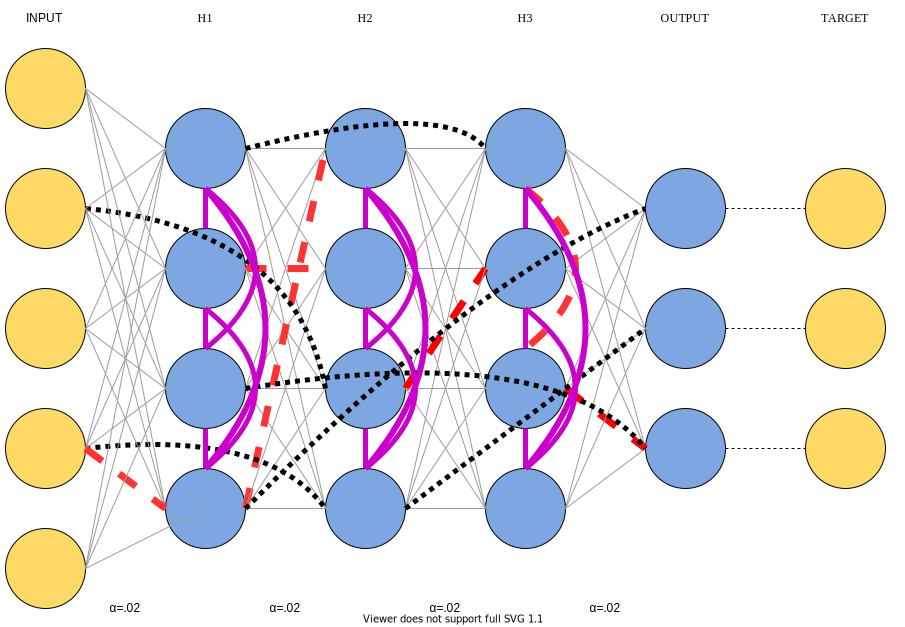
\includegraphics[width=\textwidth]{figures/topology_changes_illustration.pdf}
\end{center}
\caption{Our modifications to the topology of figure \ref{fig:top_basic} to avoid a vanishing gradient while using a global learning rate. Red dotted lines denote connections that have been removed, black dotted lines denote their replacements, and green solid lines denote added intralayer connections. All connections are bidirectional. This illustration shows a network with $p=8\%$.} \label{fig:top_sw}
\end{figure}
\begin{figure}[h!]
\begin{center}
\includegraphics[width=\textwidth]{figures/MNIST_network_comparison.pdf}
\end{center}
\caption{Performance on MNIST of the networks in section \ref{sec:implementation}. Dashed lines show the test error and solid lines show the training error. In green is a layered network with a global learning rate (section \ref{sec:basic_topology_uniform}), in orange is a layered network with per-layer rates individually tuned to counter the vanishing gradient problem (section \ref{sec:basic_topology}), and in green is a network with our topology, $p=7.56\%$ (section \ref{sec:our_topology}). Observe that our topology is almost as effective as per-layer rates at countering the vanishing gradient problem that impedes training of the layered network with a global learning rate.} \label{fig:mnist_comparison}
\end{figure}
\begin{figure}[h!]
\begin{center}
\includegraphics[width=\textwidth]{figures/MNIST_individual_layers.pdf}
\end{center}
\caption{Root-mean-square corrections to weights in different layers while training on MNIST, for the networks in section \ref{sec:implementation}. For clarity, values were subjected to an 11-point centered moving average. (left) A layered network with a single global learning rate (section \ref{sec:basic_topology_uniform}). (center) A layered network a unique, individually-tuned learning rate for each layer (section \ref{sec:basic_topology}).  (right) A network with our topology, $p = 7.56\%$ (section \ref{sec:our_topology}).Observe that the layered topology with a global learning rate has a vanishing gradient problem, which is almost completely solved by tuning an individual learning rate for each layer. Our topology improves the situation by making training uniform among the deeper layers, although the shallowest layer still trains more-quickly than the deeper layers.}   \label{fig:mnist_layers}
\end{figure}
\begin{figure}[h!]
\begin{center}
\includegraphics[width=\textwidth]{figures/MNIST_one_epoch_performance.pdf}
\end{center}
\caption{Behavior of our network (section \ref{sec:our_topology}) with varying $p$, during the first epoch of training. (top) The training error after one epoch. (bottom) Root-mean-square correction to weights in different layers during the first epoch. Observe that as $p$ is increased, the error rate decreases and the root-mean-square corrections to each layer become more-uniform.} \label{fig:mnist_1epoch}
\end{figure}

\begin{figure}[h!]
\begin{center}
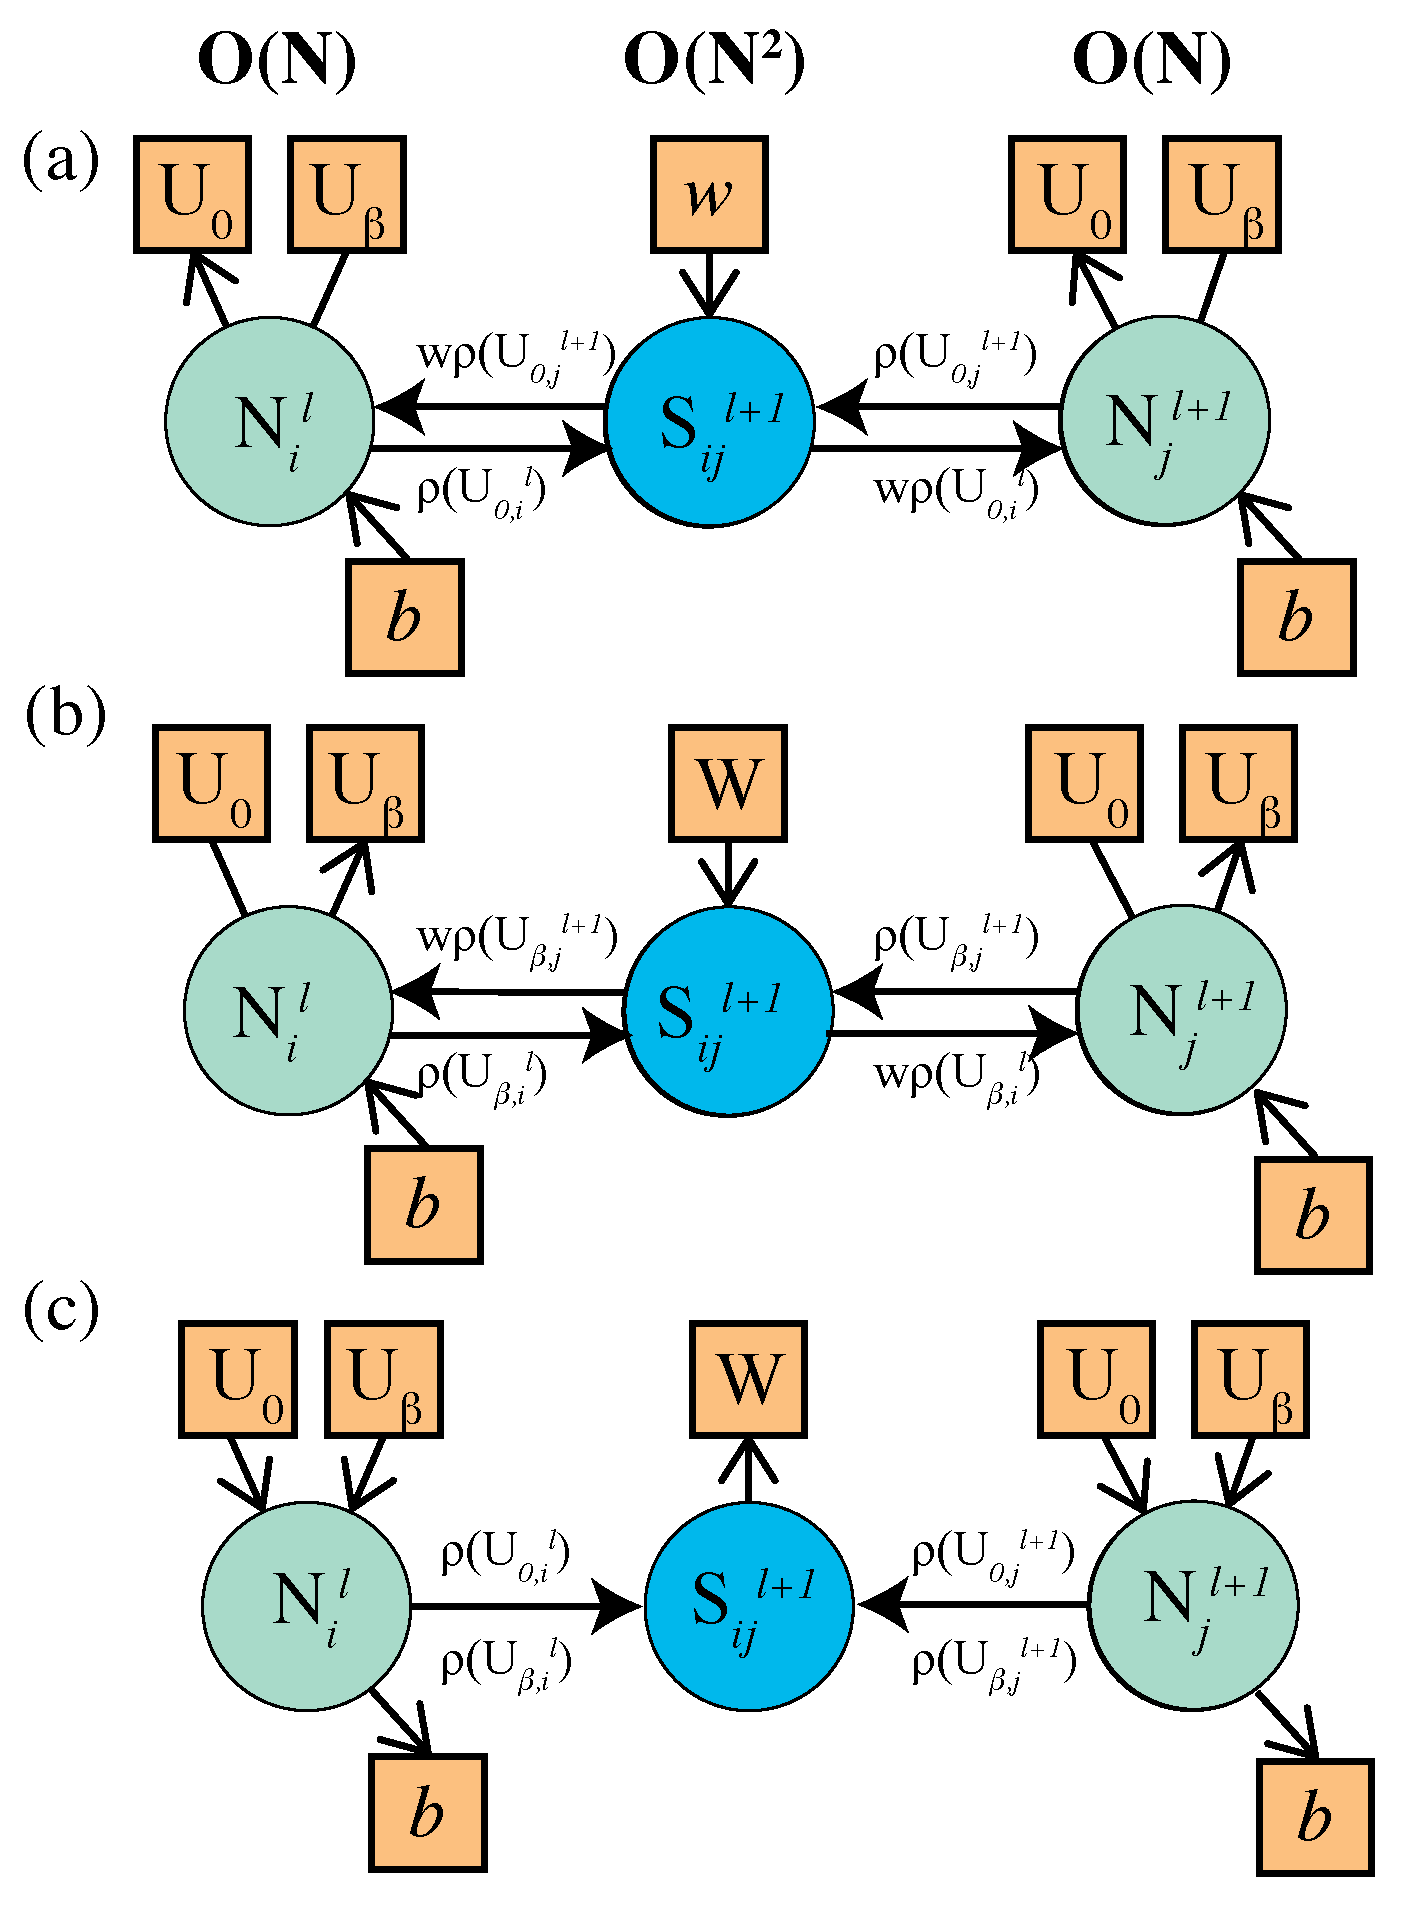
\includegraphics[width=10cm]{figures/eq_prop_sb.pdf}
\end{center}
\caption{Illustration of the functionality needed to implement equilibrium propagation in hardware. Yellow squares indicate a value that must be stored in memory for a subsequent phase. The circles indicate ($N$) neuron and ($S$) synapse devices with the associated functions described in the text. (a) The functionality required by the neurons and synapses in the free running phase. (b) The functionality of the neurons and synapses (except output neurons) in the weakly clamped phase. (c) The functionality of the neurons and synapses in the weight and bias update phase.} \label{fig:eq_prop}
\end{figure}

\begin{figure}[h!]
\begin{center}
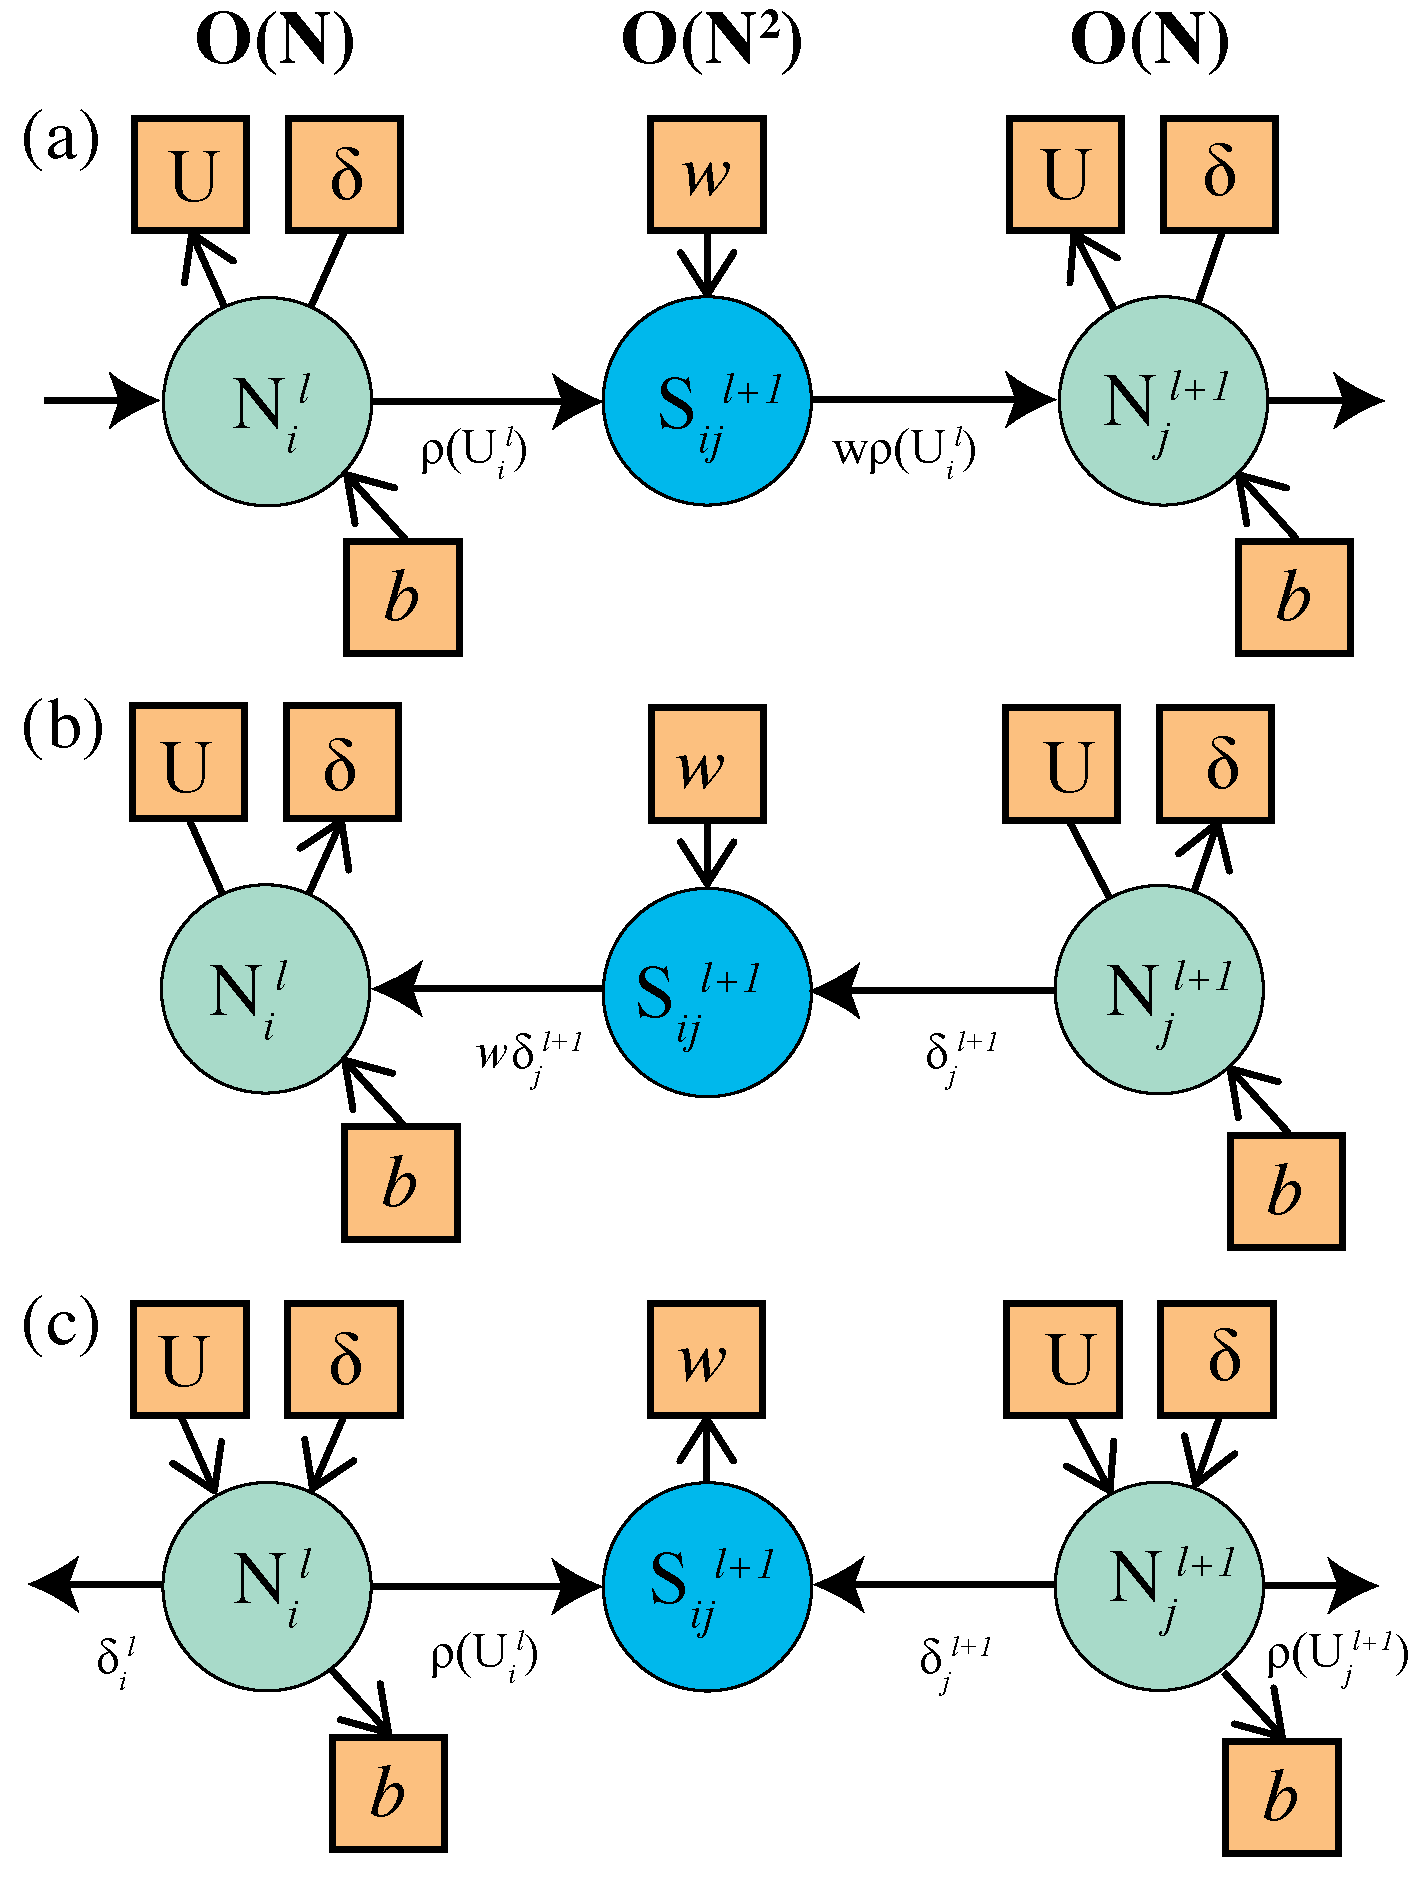
\includegraphics[width=10cm]{figures/back_prop_sb.pdf}
\end{center}
\caption{Illustration of the functionality needed to implement backpropagation in hardware. Yellow squares indicate a value that must be stored in memory for a subsequent phase. The circles indicate ($N$) neuron and ($S$) synapse devices with the associated functions described in the text. (a) The functionality required by the neurons and synapses in the forward pass phase. (b) The functionality of the neurons and synapses (except the last layer of neurons) in the backpropagation phase. (c) The functionality of the neurons and synapses in the weight and bias update phase.} \label{fig:back_prop}
\end{figure}

%\begin{figure}[h!]
%\begin{center}
%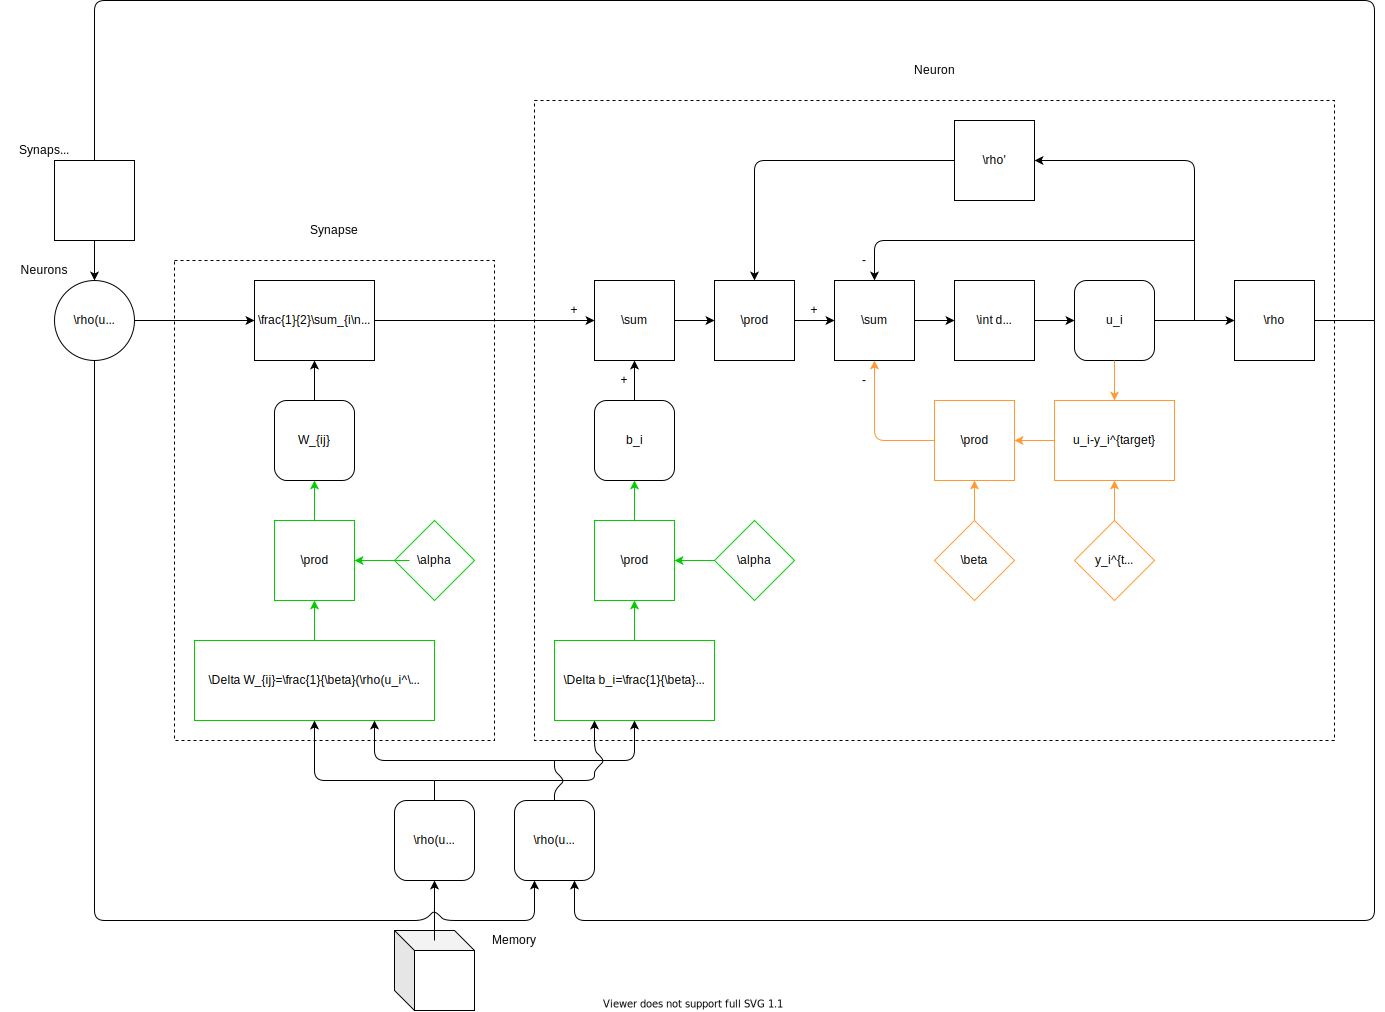
\includegraphics[width=\textwidth]{figures/eqp_bd.pdf}
%\end{center}
%\caption{Illustration of the functionality needed to implement equilibrium propagation in hardware. Black lines denote functionality needed in the free phase. Green lines denote functionality to correct parameters. Orange lines denote functionality needed only by output neurons, that is unique to the weakly-clamped phase. There is no functionality unique to the weakly-clamped phase that is needed by all neurons.} \label{fig:eqp_bd}
%\end{figure}
%\begin{figure}[h!]
%\begin{center}
%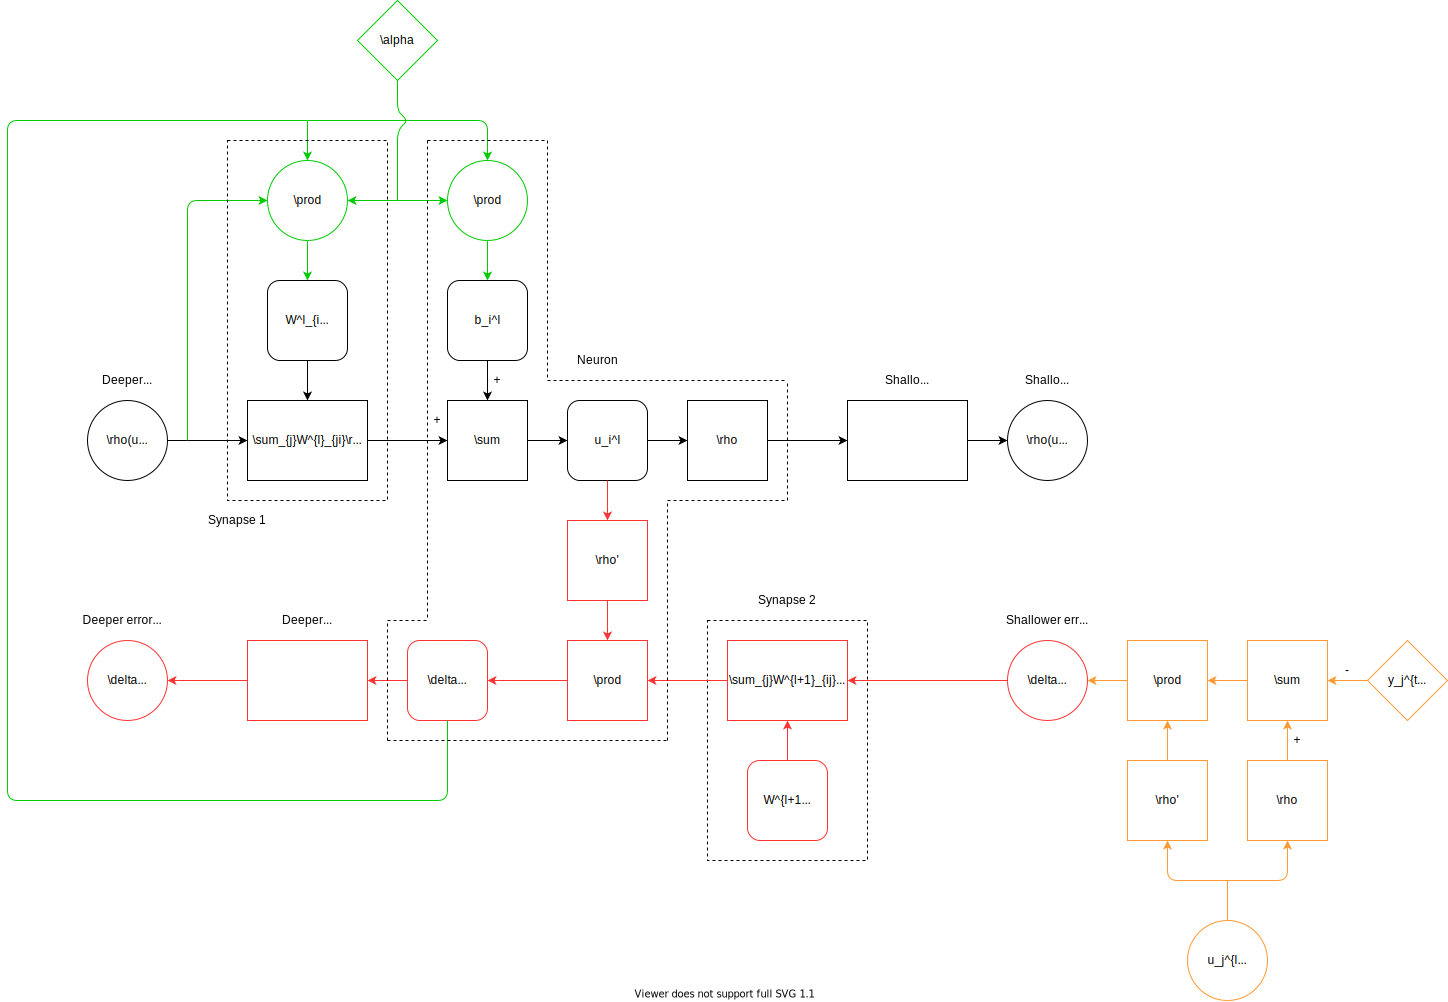
\includegraphics[width=\textwidth]{figures/backprop_bd.pdf}
%\end{center}
%\caption{Illustration of the functionality needed to implement backpropagation in hardware. Black lines denote functionality needed in the forwards phase. Green lines denote functionality to correct parameters. Red lines denote functionality unique to the backwards phase that is needed by all neurons. Orange lines denote functionality needed only by output neurons, that is unique to the backwards phase.} \label{fig:backprop_bd}
%\end{figure}
\clearpage
\section*{Tables}
\begin{table}[h!]
\begin{center}
\begin{tabular}{|L||L|L|}
\hline
&Backpropagation & Equilibrium Propagation \\ \hline\hline
Number of distinct computations & 2 -- computations during forwards and backwards phases are distinct & $\approx 1$ -- hidden neurons perform same computation in both phases. Output neurons perform a similar but modified version of the same computation. \\ \hline
Types of connections & Unidirectional to transmit activation to shallower neighbors and error to deeper neighbors & Bidirectional to each neighbor \\ \hline
Memory & Space to store activation and error term for each neuron & Space to store free and weakly-clamped activations for each neuron \\ \hline
Order of computations & Forwards propagation phase where layers are computed from deepest to shallowest; backwards propagation phase where layers are computed from shallowest to deepest; parameter update phase & Free phase where all neurons evolve simultaneously; weakly-clamped phase where all neurons evolve simultaneously; parameter update phase \\ \hline
Nonlinear activation function & Yes & Yes \\ \hline
Derivative of nonlinear activation function & Yes & Yes \\ \hline
Correction computation & Corrections require dedicated circuitry unique from that implementing propagation & Corrections require dedicated circuitry unique from that implementing evolution \\ \hline
\end{tabular}
\end{center}
\caption{Comparison of the capabilities a hardware neuron would need in order to implement backpropagation and equilibrium propagation.} \label{table:bp_eqp_contrast}
\end{table}

\end{document}
